
\chapter{Free Groups}\label{chap4} % chapter 4.

\section{}\label{chap4:sec1}

In\pageoriginale this chapter we shall consider an important class of groups called ``free
groups''. Let $E$ be a set of generation of a group $F$. We call $F$ a
free groups if $F=gp(E; \varphi)$. In other words, a free groups is
one which, in a particular set of generations, does not have any
defining relations and hence it is without non-trivial relations. An
infinite cyclic group is a free group with one generator. An immediate
consequence of Von Dyck's theorem is: 

\setcounter{theorem}{0}
\begin{theorem}\label{chap4:thm1} % them 1.
  Every mapping of the generation set $E$ of a free group $F=gp(E;
  \varphi)$ onto a group $H$ can be extended to a homomorphism of $F$
  into $H$. 
\end{theorem}

\section{Normal words}\label{chap4:sec2} % sec 2.

We now proceed to find what the elements of a free group look like. We
make the following definition 
\begin{defi*}
  \begin{enumerate}[(i)]
  \item The empty word `1' is a normal word
  \item the words $e^{m_1}_{i_1}e^{m_2}_{i_2}\cdots e^{m_ \lambda}_{i_
    \lambda}$ is a normal word if 
    \begin{enumerate}[(a)]
    \item $m_i= \pm 1$, $i=1, \ldots, \lambda$
    \item $i_j=i_{j+1}\Rightarrow m_j=m_{j+1}$.
    \end{enumerate}
  \end{enumerate}
\end{defi*}

It is clear from this definition that a normal word is one which
cannot be ``cancelled down'' to a shorter word. The number of
letters\pageoriginale 
in a word $w$ is the \textit{length} if the word $w$ and is denoted by
$\lambda(w)$. We put $\lambda(1)=0$. 

The following theorem shows that any word can be cancelled down to a
unique normal word. 

\begin{theorem}\label{chap4:sec2:thm2}% Them 2.
  Every word is trivially equal (i.e. equal by a trivial relation) to
  a normal word and this normal word is unique. 
\end{theorem}

\begin{proof}
  We prove the first part of the theorem by induction on the
  length. Let $G=gp(E)$ be a group and let $w(e)$ be a word in $E$,
  with $\lambda(w)=n$. When $n=0$, by definition $w$ is the empty word
  and hence normal. Thus the theorem is true for $n=0$. Assume that
  every word $v$, with $\lambda (v)<n$, is 'trivially equal' to a
  normal word. Let \footnote{We use $\equiv$ for equality of words,
    $=$ for equality of group elements}
  $w=e^{m_1}_{i_1}e^{m_2}_{i_2}\cdots e^{m_n}_{i_n}$ and thus $\lambda
  (w)=n$. 
\end{proof}

If $w$ is normal, there is nothing to prove. If $w$ is not normal,
then there is a positive integer $j$ such that
$i_j=i_{j+_1},m_j=-m_{j+1}$. Put $u=e^{m_1}_{i_1}e^{m_2}_{i_2}\cdots$ 
$e^{m_{j-1}}_{i_{j-1}}, u'=e^{m_{j+2}}_{i_{j+2}} \cdots
e^{m_n}_{i_n}$. Then $w \equiv
ue^{m_j}_{i_j}e^{m_{j+1}}_{i_{j-1}},u'$. It is immediate that $w
\equiv ue^{m_j}_{i_j}e^{m_{j+1}}_{i_{j-1}},u'=uu' \equiv v$ is a
trivial relation. But $\lambda (v)=n-2$. Therefore induction
hypothesis, there is a normal word $w'$ such that $v=w'$ is a trivial
relation. Since $w=v$ is also a trivial relation it follows by
transitivity that $w=s'$ is a trivial relation. This
proves\pageoriginale the first part of the theorem. 

We say that word $v$ is obtained from the word $u$ by an
\textit{`elementary reduction'} if there is a `letter' $e$ in $u$ such
that $u \equiv u'e^m e^{-m}u''$ and 
$$
v \equiv u' u'',m= \pm 1.
$$

To prove the uniqueness we required the following two lemmas.

\begin{lem}\label{chap4:sec2:lem1}%lemma 1.
  Two words $v,v'$ are trivially equal (i.e. $v=v'$ is a trivial
  relation) if and only if there is a finite sequence of words
  $v=v_0$, $v_1, \ldots, v_n=v'$, such that for every $i(1 \leq i \leq
  n)$, either $v_{i+1}$ is got from $v_i$ by elementary reduction or
  $v_i$ is got from $v_{i+1}$ by elementary reduction. 
\end{lem}

\begin{lem}\label{chap4:sec2:lem2}% lemma 2.
  (The ``Diamond Lemma''). If $u_1$ and $u_2$ are obtained from the
  same word $v$ by elementary reduction, then either $u_1 \equiv u_2$,
  or each can be reduced by an elementary reduction to one and the
  same word $v^*$.  
\end{lem}

\begin{proof}
  Let
  
  \noindent 
  \begin{minipage}[c]{6cm}
    \begin{align*}
      v & =e^{m_1}_{i_1}e^{m_2}_{i_2}\cdots e^{m_n}_{i_n},\\
      i_j &=i_{j+1},m_j =-m_{j+1},\\
      i_k &= i_{k+1},m_k=-m_{k+1},
    \end{align*}
    and $u_1$ obtained by omitting $e^{m_1}_{i_1}e^{m_{j+1}}_{i_{j+1}}$
    from $v$, and $u_2$ by omitting $e^{m_k}_{i_k}e^{m_{k+1}}_{i_{k+1}}$,
    where we may without loss of generality suppose that $j \leq k$.  
  \end{minipage}
  \begin{minipage}[c]{4cm}
    \begin{figure}[H]
      \centering{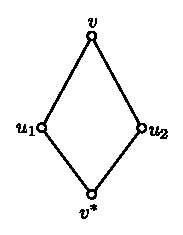
\includegraphics{vol21-figures/fig21-1.eps}}
    \end{figure}
  \end{minipage}

  Then\pageoriginale if $j=K$, then $u_1 \equiv u_2$ (trivially).
\end{proof}

If $j=k-1$, then $e^{m_j}_{i_j}e^{m_{k+1}}_{i_{k+1}}=e^m$, say, and 
$$
u_1 \equiv e^{m_1}_{i_1}\cdots
e^{m_{j-1}}_{i_{j-1}} \,e^m \, e^{m_{k+2}}_{i_{k+2}}\cdots e^{m_n}_{i_n}\equiv
u_2. 
$$

Finally, if $j <k-1$, put
$$
v^*=e^{m_1}_{i_1}\cdots e^{m_{j-1}}_{i_{j-1}}e^{m_{j+2}}_{i_{j+2}}
\cdots e^{m_{k-1}}_{i_{k-1}} e^{m_{k+2}}_{i_{k+2}} \cdots
e^{m_n}_{i_n}. 
$$

Then $v^*$ is obtained from $u_1$ by the elementary reduction that
deletes $e^{m_k}_{i_k}e^{m_{k+1}}_{i_{k+1}}$ and from $u_2$ by
similarly deleting $e^{m_j}_{i_j} e^{m_{j+1}}_{i_{j+1}}$. 

We now give an intuitive argument to show that if two normal words are
trivially equal, then they are identical. Let $w,w'$ be two words such
that $w = w'$ is a trivial relation. By lemma \ref{chap4:sec2:lem1},
there exists words 
$w=v_0,v_1, \ldots, v_n=w'$ such that either $v_{i+1}$ is obtained
from $v_i$ by elementary reduction or vice versa, for $i=0,1, \ldots
,n$. In the following figure we write $v_{i+1}$ above $v_i$ and
connect it to $v_i$ if $v_{i+1}$ is obtained from $v_i$ by elementary
reduction. 

\begin{figure}[H]
  \centering{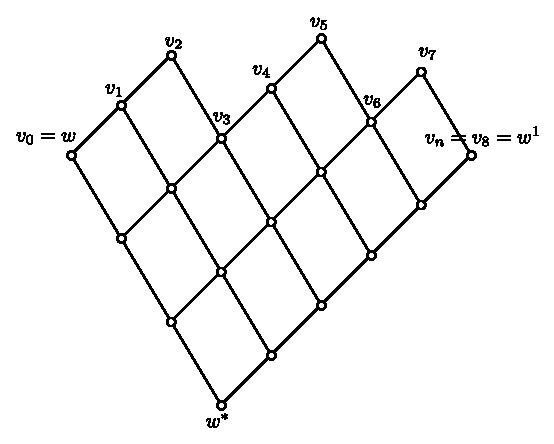
\includegraphics{vol21-figures/fig21-2.eps}}
\end{figure}

A\pageoriginale glance at the above figure shows that by several applications of the
diamond lemma, we descend down to a word $w^*$, which is trivially
equal to $w$ and $w'$, or $w$ and $w'$ are identical. Now if $w$ and
$w'$ are normal words which are trivially equal, then they have to be
identical as further descent is not possible. 

A\pageoriginale formal proof of the above lemma can be found in M.H.A
Newman (1942). 
\begin{coro*}
  If $G=gp(E)$, then every element $g \in G$ has a representation
  $g=w(\underbar{e})$ where $w$ is normal. 
\end{coro*}

In particular in a free group, every element is representative by one
and only one normal word. This follows from the fact that in a free
group there are no non-trivial relations. 

\section{}\label{chap4:sec3}% sec 3

Let $G$ be any group with $G=gp(E; R)$ and $F=gp(E^0, \varphi)$ a free
group such that $|E^0|=|E|$. There is a mapping $\varphi$ of $E^0$
onto $E$ which is one-one. By Von Dyck's theorem $\varphi$ can be
extended to an epimorphism $\varphi^*$ of $F$ onto $G$. 

Let $N=\{ 1 \}^{\varphi *^{-1}}$ be the kernel of $\varphi^*$. Then $N
\Delta F$. Let $f \in F$. Then $f=w(\underbar{e}^0)$. Without loss of
generality we can assume that $w$ is a normal word. We have 
$$
\displaylines{\hfill 
  f^{\varphi^*}=w(\underbar{e})=g \in G \hfill \cr
  \text{where}\hfill e^0=(e^0_1, \ldots, e^0_n)\hspace{1cm}\hfill \cr
\hfill   e^0=(e_1, \ldots, e_n) \text{ and } e_i=e^{\circ^\varphi}_i.\hfill}
$$

Now $f \in N$ if and only if $g=1$; i.e., $f \in N$ if only if
$w(\underbar{e})=1$ is a relation in $G$. Since any relation of $G$ can
be written in the form $w=1$, it follows that $N$ completely
determines the relation in $G$. Hence $N$ is called the
\textit{relation group} of $G$. 

Further\pageoriginale
$$
g \cong F/N.
$$
Thus we have the following theorem.

\begin{theorem}\label{chap4:sec3:thm3}%Thm 3
  Every group is an epimorphic image of a free group and hence is
  isomorphic to a quotient group of a free group. 
\end{theorem}

If a set of defining relation $R$ of $G$ is given we can say something
more about the structure of $N$. Let $R=\{ f_i \equiv w_i
(\underbar{e})=1 \bigg| i \in I \}$ be a set of defining relations of
$G$. Without loss of generality we can assume that all $w_i
(\underbar{e})$ are normal words. We claim that $N$ is the normal
closure in $F$ of $\{ f'_i\}_{i \in I}$, where
$f'_1=w_i(\underline{e^0})$. That is to say $N$ is the normal subgroup
of $F$ containing $\{ f'_1 \}_{i \in I}$. In other words, if $R'=\{
f'_1 \}_{i \in I}$, then 
$$
N=\bigcap_{R' \subseteq M \Delta F} M
$$

Since $R' \subseteq N \Delta F$, we have $N' \subseteq N$, where $N'$
denotes the normal closure of $R'$. Consider now the quotient
$F/N'$. All the defining relations $w_i=1,i \in I$ of $G$, are
satisfied in $F/N'$ as $R' \subseteq N'$. Hence any relation $w=1$
satisfied in $G$ is also satisfied in $F/N'$. Let $f \equiv w(e^0)\in
N$. Then $w(e)=1$ is a relation in $G$ and therefore
$w(e^0)N'=N'$. i.e., $w(e^0)\in N'$. Hence $N \subseteq N'$.  

In virtue of the reversed inclusion which we already have, this proves
that $N=N'$. 

The\pageoriginale following theorem gives a method of construction for $N'$.

\begin{theorem}\label{chap4:sec3:thm4}% Them 4
  Let $G$ be any group, $S \subseteq G$. Then the normal closure $T$ of
  $S$ in $G$ is the totality of all elements $t$ of the form 
  $$
  t=g^{-1}_1 s^{m_1}_1 g_1 g^{-1}_1 s_2^{m_2}g_2 \cdots g^{-1}_
  \lambda s_ \lambda^m g_ \lambda,
  $$
  where $m_i=\pm1, \lambda$ arbitrary, $g_i,s_i$ are arbitrary
  elements of $G$ and $S$ respectively. 
\end{theorem}

\begin{proof}
  Let $T$ denote the totality of such elements. Trivially $T$ is
  contained in the normal closure of $S$. To complete the proof of the
  theorem, we have only to show that $T \Delta G$. That $T$ is closed
  under right division is easy to verify, so that $T \leq G$. If $g
  \in G$, then  
  \begin{align*}
    g^{-1}tg &=g^{-1} g^{-1}_1 s_1^{m_1} g_1 g_2^{-1} s_2^{m_2} g_2 \cdots g^{-1}_
    \lambda s_\lambda^m g_\lambda g\\ 
    &= (g_1 g)^{-1} s^{m_1}_1 (g_1 g) \,(g_1
    g)\, (g_2 g)^{-1} s_2^{m_2} (g_2 g)\cdots (g_\lambda g)^{-1} s^{m} 
    (g_\lambda g) \in T 
  \end{align*}
  for arbitrary  $t \in T$. Therefore $T \Delta G$. Hence the theorem.
  Determining to our $N$, we see that $N$ consists of all elements of
  the form 
  $$
  t^{-1}_1 w^{\pm 1}_{i_1}t_1t_2^{-1}w^{\pm 1}_{i_2} t_2 \cdots t_
  \lambda^{-1}w^{\pm 1}_{i_\lambda}, \text{ where } 
  $$
  $t_ \lambda 's$ are arbitrary and $w_{i_k}\in R'$.
\end{proof}

\section{Dual property of free groups}\label{chap4:sec4} % sec 4.

\begin{theorem}\label{chap4:sec4:thm5}% Them 5.
  If a group $G$ is epimorphically mapped on a free group $F$, then
  $G$ contains a free subgroup isomorphic to $F$, and in fact mapped
  isomorphically\pageoriginale onto $F$ by the restriction to it of the epimorphism
  of $G$. 
\end{theorem}

\begin{proof}
  Let $\varphi$ be an epimorphism of $G$ onto $F$. Let
  $F=gp(E,\varphi)$. Then $e^{\varphi^{-1}}$ is a non-empty for every $e
  \in E$. Choose an $e_1$ from $e^{\varphi^{-1}}$. Denote by $E_1$
  the set of all such $e_1's$. Let $F_1=gp(E_1)$. We claim that the
  restriction $\varphi_1$ of $\varphi$ to $F_1$ ia an isomorphism of
  $F_1$ onto $F$. That the
  mapping $\varphi_1$ is an epimorphism is obvious, by our choice of
  $e_1's$. Now if $g \in F$, let $w(\underbar{e})$ he a normal word
  representing $g$. Then
  $g^{\varphi_1}=(w(\underbar{e}))^{\varphi_1}=(w(\underbar{e}))^{\varphi}=
  (w(\underbar{e}^\varphi
  _1))=w(\underbar{e})=1$ if and only if $w$ is the empty word, as $F$
  is a free group. Hence the kernel of $\varphi _1$ consists of the
  neutral elements alone and therefore $\varphi_1$ is an
  isomorphism. Since any group isomorphic to a free group is also
  free, our theorem follows. 
\end{proof}

\begin{theorem}\label{chap4:sec4:thm6}%THEM 6.
  Free groups generated by sets of the same cardinality are isomorphic.
\end{theorem}

\begin{proof}
  Let $E$ and $E^0$ be two sets such that $|E|=|E^0|$, $F=gp(E,\phi)$
  and $F^0=gp(E^0, \phi)$. Let $\psi$ be a one-one mapping of $E^0$
  onto $E$. Extend it to an epimorphism of $F^0$ onto $F$. We shall
  also denote this extended mapping by $\psi$. 
\end{proof}

Now $(w(c^\circ))^\psi=w(e)=1$ if and only if $w$ is an empty word. This
follows because we can without loss of generality take $w$ to be a
normal word. hence $w(e^0)=1$. Therefore $\psi$ is an isomorphism of
$F^0$ onto $F$. 

This\pageoriginale shows that the structure of a free group depends only on the
cardinality of its set of generators. We call $|E|$ the rank of the
free group $gp(E, \phi)$. A free of rank zero is the trivial group $\{
1 \}$. Free groups of rank $1$ are finite cyclic groups. 

It is natural to ask if free groups of different ranks are in fact
different. The following theorem answer this question. 

\begin{theorem}\label{chap4:sec4:thm7} %Them 7
  Free groups of different ranks are not isomorphic.
\end{theorem}

To prove this theorem we need the following lemma, the proof of which
we shall give later. 
\begin{lemma*}
  To every cardinal number $n$ there is group $G_n$ that can be
  generated by a set of cardinal $n$ elements, but by no set of
  strictly smaller cardinal. 
\end{lemma*}

\noindent \textbf{Proof of the theorem.} 
  Let 
  \begin{align*} 
    F_n &= gp(E_n, \phi), |E_n| =n,\\ 
    F_m &=gp(E_m, \phi), |E_m| =m 
  \end{align*}
  where $n$ and $m$ may be infinite cardinals. Choose $G_n$ of the
  above lemma. Then there is a epimorphism $\psi$ of $F_n$ onto
  $G_n$. Assume that there is an isomorphism 
  $\varphi$ of $F_m$ onto $F_n$. Then $\varphi \psi$ is an
  epimorphism of $F_m$ onto $G_n$.  Therefore $E_m^{\varphi \psi}$
  generates the group $G_n$. Hence we have $m=|E_m|\geq |E_m^{\varphi
    \psi}|\geq n$ using the isomorphism $\varphi^{-1}$, we similarly
  get $n \geq m$. Hence $m=n$. Differently put, $F_m$ and $F_n$ are
  not isomorphic if $m \neq n$. Hence the theorem.  
 
\noindent\textbf{Proof of the lemma.}
  For every cardinal $n$, we shall construct a $G_n$ with the desired
  property. Let $M$ be any set with $|M|=m$. Consider the\pageoriginale set $G$ of
  all finite subsets of $M$. We turn $G$ into a group by defining the
  binary operation as the symmetric difference. That is to say, for
  every $S,T \in  G$. 
  $$
  ST=(S-T)\bigcup (T-S)
  $$
  We take the empty set $\phi$ as the unit element and each $S$ as its
  own inverse. For we have 
  $$
  S \phi=\phi S=S \text{ and }SS=\phi, \text{ for every } S \in  G.
  $$

  The verification of the associativity of this multiplication is easy
  and therefore we omit it. Hence the multiplication defined in $G$,
  makes $G$ a group. We  claim that this group $G$ is generated by the
  set of one-element subsets of $M$, $E= \bigg \{ \{ x\} \bigg | x \in
  M \bigg \}$. For if $S=\bigg \{ a_1,a_2, \ldots, a_k \bigg \}$, it
  is easily seen that $S=\{ a_1\} \{ a_2\} \cdots \{ a_k \}$. Further
  for every $S$, $T \in  G$, we have $ST=TS$. Therefore $G$ is
  commutative. We shall show that no set of cardinal $<m$ generates
  $G$. Let $E^0$ be a set of generators of $G$ with $E^0=n$, say. Then
  every elements $x \in  G$ can be written as 
  $$
  x=s^{m_1}_1 S^{m_2}_2 \cdots S^{m_k}_k \text{ with } m_i=\pm1, S_i
  \in  E^0, i=1,\ldots, k. 
  $$

  But in $G$, we have $S=S^{-1}$, for every $S \in 
  G$. Therefore every $x \in  G$, can be written as 
  $$
  x=S_1S_2 \cdots S_k \text{ with district generators } S_i \in  E^0.
  $$
  
  Further,\pageoriginale since $G$ is commutative it follows that every finite
  subset of $E^0$ determines only one element of $G$. Thus to every
  element $x \in  G$, we can associated a finite subset of
  $E^0$. This shows that $|G|\leq$ cardinal of the set of all finite
  subsets of $E^0$. But we know that if $X$ is any set and $F$ the set
  of all finite subset of $X$. Then 

\noindent $\begin{aligned}
    & |F|= 2^X \text{ if }|X|< \mathcal{N}_0\\
    \text{ and } \hspace{3cm} &|F|= X \text{ if }|X|\geq \mathcal{N}_0
  \end{aligned}
$

  Thus if $m$ is finite, we have, from the above inequality, that $2^m
  \leq 2^n$, and therefore $m \leq n$. If $m$ is infinite and $n$ is
  finite, we have $m \leq 2^n$, which is impossible. Hence if $m$ is
  infinite, $n$ must also be infinite, and again conclude that $m \leq
  n$. Hence the group $G$ cannot be generated by a set of cardinals
  strictly smaller than $m$. This establishes the lemma. 

